\documentclass[aspectratio=1610]{beamer}
\usepackage{graphicx}
\usepackage{amssymb,amsmath,amsfonts}
\usepackage[spanish,es-tabla]{babel}
\usepackage[ansinew]{inputenc}
\usepackage{xcolor}
%\usepackage{enumitem}
\usetheme{Madrid} 
\useinnertheme{circles}
\usecolortheme{default} 

\setbeamercolor{structure}{fg=green!60!black} % Color principal a un tono de verde
\setbeamercolor{title}{fg=green!60!black} % Establece el color del t�tulo al verde
\setbeamercolor{subtitle}{fg=green!50!black} % Establece el color del subt�tulo al verde

\usefonttheme[onlymath]{serif} % Cambiar a fuente serif para matem�ticas
%\usefonttheme{serif}

\title{\bf Regresi�n Lineal}
\subtitle{Consideraciones para el an�lisis de datos en los cursos de laboratorio de F�sica}
\author{H�ctor F. Hern�ndez G.}
\date{\today}

% Definir el color verde personalizado
\definecolor{customgreen}{RGB}{0,128,0}

% Configurar los colores de Beamer para el tema Warsaw
\setbeamercolor{title in head/foot}{bg=customgreen, fg=white}
\setbeamercolor{author in head/foot}{bg=customgreen, fg=white}
\setbeamercolor{date in head/foot}{bg=customgreen, fg=white}
\setbeamercolor{section in head/foot}{bg=customgreen, fg=white}
\setbeamercolor{subsection in head/foot}{bg=customgreen, fg=white}
\setbeamercolor{frametitle}{bg=customgreen, fg=white}
\setbeamercolor{block title}{bg=customgreen, fg=white}
\setbeamercolor{block body}{bg=customgreen!10, fg=black}
\setbeamercolor{item}{fg=customgreen}


\begin{document}
\frame{\titlepage}

\begin{frame}
\frametitle{Objetivos del Cap�tulo}
\begin{itemize}
    \item Obtener Mediciones Precisas
    \item Elaboraci�n y An�lisis de Gr�ficos
    \item Redacci�n de Informes de Laboratorio
    \item Exploraci�n de Nuevos T�picos de la F�sica
\end{itemize}
\end{frame}

\begin{frame}
\frametitle{Sistema Internacional de Unidades (SI)}
\begin{table}[]
    \centering
    \begin{tabular}{ccc}
        \hline
        \textbf{S�mbolo} & \textbf{Nombre} & \textbf{Magnitud} \\ \hline
        s & segundo & tiempo \\
        m & metro & longitud \\
        kg & kilogramo & masa \\
        A & amperio & corriente el�ctrica \\
        K & kelvin & temperatura termodin�mica \\
        mol & mol & cantidad de sustancia \\
        cd & candela & intensidad luminosa \\ \hline
    \end{tabular}
\end{table}
\end{frame}

\begin{frame}
\frametitle{Instrumentos de Medici�n}
\begin{itemize}
    \item Masa: Balanzas
    \item Longitud: Cinta m�trica, Vernier, Tornillo Microm�trico
    \item Tiempo: Cron�metro
    \item Temperatura: Term�metro
    \item Corriente El�ctrica: Amper�metro
    \item Cantidad de Sustancia: Mol
    \item Intensidad Luminosa: Lux�metro
\end{itemize}
\end{frame}

\begin{frame}
\frametitle{Medici�n de la Masa}
\begin{itemize}
    \item Unidad: Kilogramo (kg)
    \item Instrumentos: Balanza de dos platillos, balanza de un solo platillo, balanza anal�tica
\end{itemize}
\end{frame}

\begin{frame}
\frametitle{Medici�n de la Longitud}
\begin{itemize}
    \item Unidad: Metro (m)
    \item Instrumentos: Cinta m�trica, Vernier, Tornillo Microm�trico
\end{itemize}
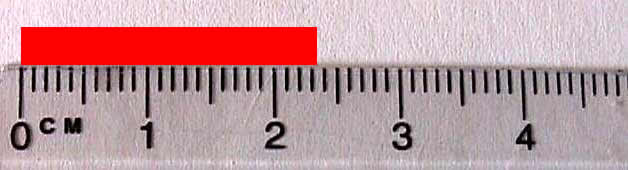
\includegraphics[width=0.8\textwidth]{figuras/fig02a}
\end{frame}

\begin{frame}
\frametitle{Medici�n del Tiempo}
\begin{itemize}
    \item Unidad: Segundo (s)
    \item Instrumento: Cron�metro (digital y anal�gico)
\end{itemize}
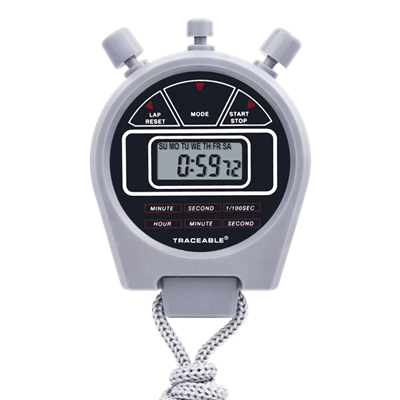
\includegraphics[width=0.4\textwidth]{figuras/fig02f1}
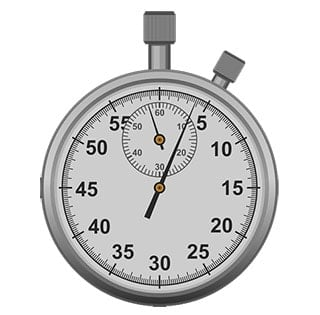
\includegraphics[width=0.4\textwidth]{figuras/fig02f2}
\end{frame}

\begin{frame}
\frametitle{Medici�n de la Temperatura}
\begin{itemize}
    \item Unidades: Celsius (�C), Fahrenheit (�F), Kelvin (K)
    \item Instrumentos: Term�metros (anal�gicos y digitales)
\end{itemize}
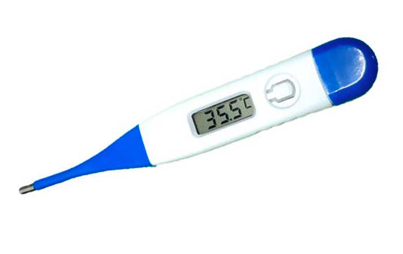
\includegraphics[width=0.4\textwidth]{figuras/fig02g2}
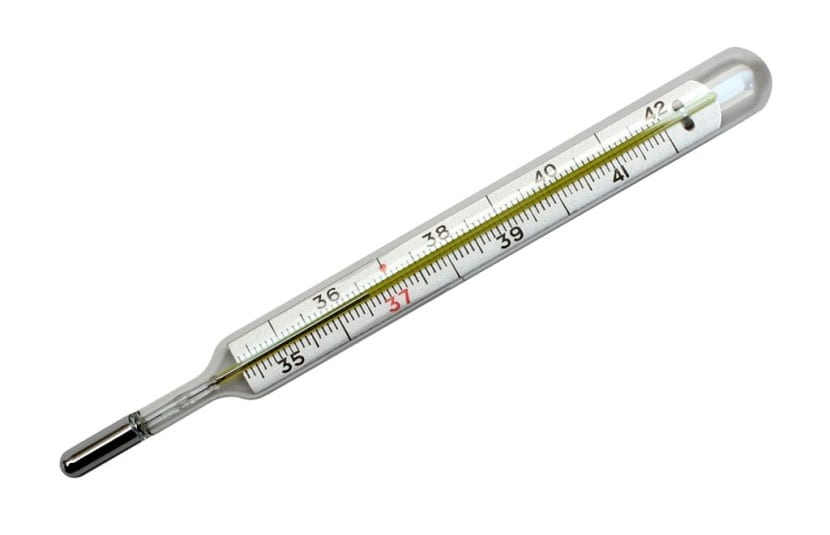
\includegraphics[width=0.4\textwidth]{figuras/fig02g1}
\end{frame}

\begin{frame}
\frametitle{Medici�n de la Corriente El�ctrica}
\begin{itemize}
    \item Unidad: Amperio (A)
    \item Instrumento: Amper�metro
\end{itemize}
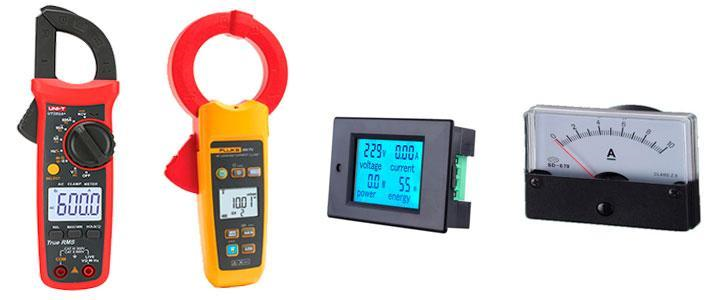
\includegraphics[width=0.8\textwidth]{figuras/fig02h}
\end{frame}

\begin{frame}
\frametitle{Medici�n de la Cantidad de Sustancia}
\begin{itemize}
    \item Unidad: Mol (mol)
    \item Definici�n: Relaci�n entre el n�mero de entidades elementales y la constante de Avogadro
\end{itemize}
\end{frame}

\begin{frame}
\frametitle{Medici�n de la Intensidad Luminosa}
\begin{itemize}
    \item Unidad: Candela (cd)
    \item Instrumento: Lux�metro
\end{itemize}
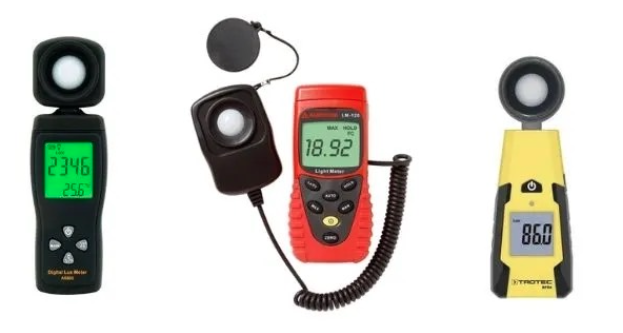
\includegraphics[width=0.8\textwidth]{figuras/fig02i}
\end{frame}

\end{document}